%%%%%%%%%%%%%%%%%%%%%%%%%%%%%%%%%%%%%%%%%%%%%%%%%%%
%% FUNCIÓN PARA INCLUIR UNA FOTO EN EL DOCUMENTO %%
%%%%%%%%%%%%%%%%%%%%%%%%%%%%%%%%%%%%%%%%%%%%%%%%%%%

\begin{figure}[thbp]
%Se comienza a escribir esta función para crear el entorno de imágenes. Los argumentos opcionales indican donde se coloca la foto que vas a añadir. Es decir, que se escriba estas función después de un texto no implica que se incluyan las fotos después de dicho texto sino que LATEX las colocará donde mejor queden, según la distribución de espacio (y siendo la primera opción donde has indicado). Aún así, en caso de que se cambien de sitio de forma automática, se puede forzar para que se incluyan en un sitio determinado o que se vaya buscando los sitios que mejor convengan según un orden. Los parámetros son: “t”=“top” es decir, al principio de la página en la que está escribiendo, “h”=“here” es decir justo aquí (después del correspondiente párrafo), “b”=“bottom” es decir, al final de la página en cuestión o “p”=“page” es decir, en la siguiente página. Para forzar y que sí o sí se incluya la foto donde se quiere habrá que escribir [H] en mayúsculas, y para que esto funcione habrá que previamente haber incluido al inicio del documento el paquete “Float”. 

\centering
%Función que indica que la foto se deberá encontrar centrada con respecto al texto, es decir, en medio de la página.

\fbox{
\includegraphics[width=0.7\textwidth, height=3.8cm]{Figuras/LDeusto.jpeg}}
%Esta es la función propiamente dicha que incluye la foto que queremos incluir en la memoria. Va por partes.

%Lo primero de todo, la función "\fbox" se utiliza para crear un recuadro negro alrededor de la foto (si no se quiere recuadrar simplemente se elimina dicha función). 

%Posteriormente "\includegraphics" es la función que propiamente llama a la imagen correspondiente. El argumento obligatorio de includegraphics es la dirección y el nombre de tu foto (que está previamente cargada en el menú de tu proyecto) junto con el formato utilizado (.png, .PNG, .jpg)...

%Los parámetros opcionales sirven para dar dimensiones a la imagen que se quiere insertar. En este caso, se determina que la imagen ocupe el 70% de la distancia que ocupa el texto, y además se indica que la altura de la imagen sea exactamente de 3.8 centímetros. Evidentemente estos parámetros variarán en función de la foto a incluir y en función de las preferencias del estudiante.

\caption{Logo: Universidad de Deusto (Fuente: Deusto \cite{Deusto}).}
%La función "\caption" permite añadirle a la foto un subtítulo en el que por ejemplo se puede incluir el nombre de la foto y la fuente de procedencia. 

\label{fig:Deusto}
%Al igual que los capítulos, a las fotos también se les añade una etiqueta correspondiente para poder referenciarlas. Para añadir la etiqueta simplemente se utiliza la función "\label" y se le indica como parámetro obligatorio la etiqueta correspondiente.

\end{figure}
%Finalmente se cierra el entorno de imagen.

%%%%%%%%%%%%%%%%%%%%%%%%%%%%%%%%%%%%%%%%%%%%%%%%
%% FUNCIÓN PARA INCLUIR DOS FOTOS EN PARALELO %%
%%%%%%%%%%%%%%%%%%%%%%%%%%%%%%%%%%%%%%%%%%%%%%%%

%El proceso para incluir dos fotos en paralelo es muy similar a incluir una única foto, sólo que con algunas diferencias que se exponen a continuación.

\begin{figure}[ht]
%Se inicia el entorno figura.

\centering
%Se centran las dos fotos es decir, parten desde el centro.

\begin{minipage}[h]{.48\linewidth}
%Esta es la primera función diferente. Para incluir dos fotos es necesarios crear en el documento una especie de dos "minipáginas" una paralela a otra. Esta minipáginas son donde se incluirá cada una de las fotos respectivamente. Para ello se crea esta función y se indica que la primera minipágina a crear ocupe el 48% de la longitud del texto (modificable en función de las dimensiones de la foto).

\vspace{1.5cm}
%Esta función la veremos al acabar.

\fbox{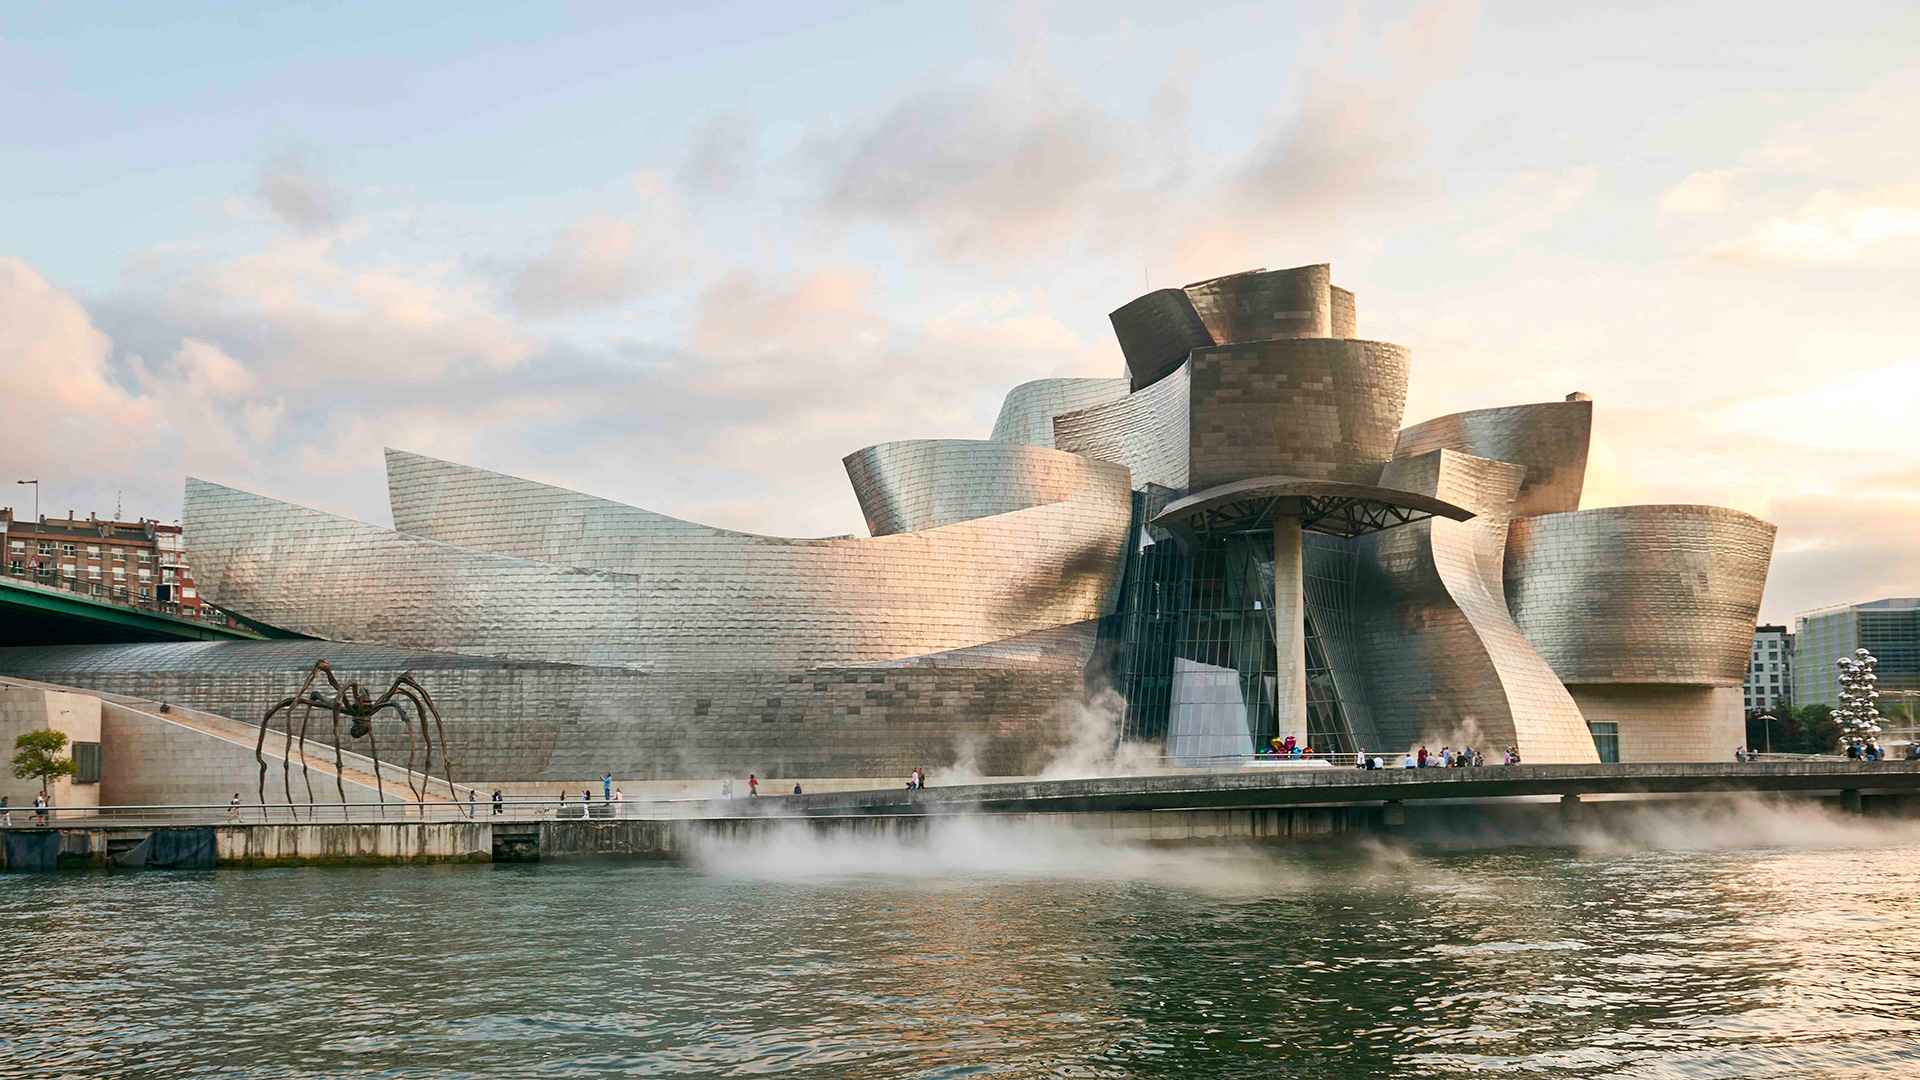
\includegraphics[width=\textwidth, height=4.5cm]{Figuras/Gugg.jpg}}
%A continuación nuevamente se incluye la foto de la misma manera que si fuese una única foto. A diferencia de antes, cuando se indica que la foto ocupe el 100% de la longitud del texto, no es el texto global del documento sino el texto de la minipágina en cuestión. Esto significa que la foto ocupe el 100% del 48% que ocupa la minipágina, es decir, que ocupe la minipágina creada al completo.

\caption{Guggenheim - Bilbao (Fuente: Google \cite{Gugg}).}
%Nuevamente se le añade un subtítulo a la foto y su correspondiente fuente.

\label{fig:Gugg}
%Se añade la etiqueta de la foto.

\end{minipage}
%Se cierra la minipágina creada.

\hfill
%Esta función es muy importante y determinará la separación entre las fotografías y las minipáginas en posición horizontal. Así, la función "\hfill" indica que independientemente  de cuales sean los anchos de las fotos, se quiere que ambas estén justificadas con el texto. Es decir, que se rellene la distancia en el medio para que la foto de la izquierda quede lo más a la izquierda posible y la de la derecha, lo más a la derecha posible.

%Si no se quiere que las fotos se justiquen totalmente, se puede utilizar la función "\hspace{20mm}" que indica que las fotos partan desde el centro del documento y que la distancia entre sus bordes sea exactamente 20 milímetros (o la distancia que se indique)

\begin{minipage}[h]{.45\linewidth}
%Se crea la nueva minipágina (la de la derecha).

\fbox{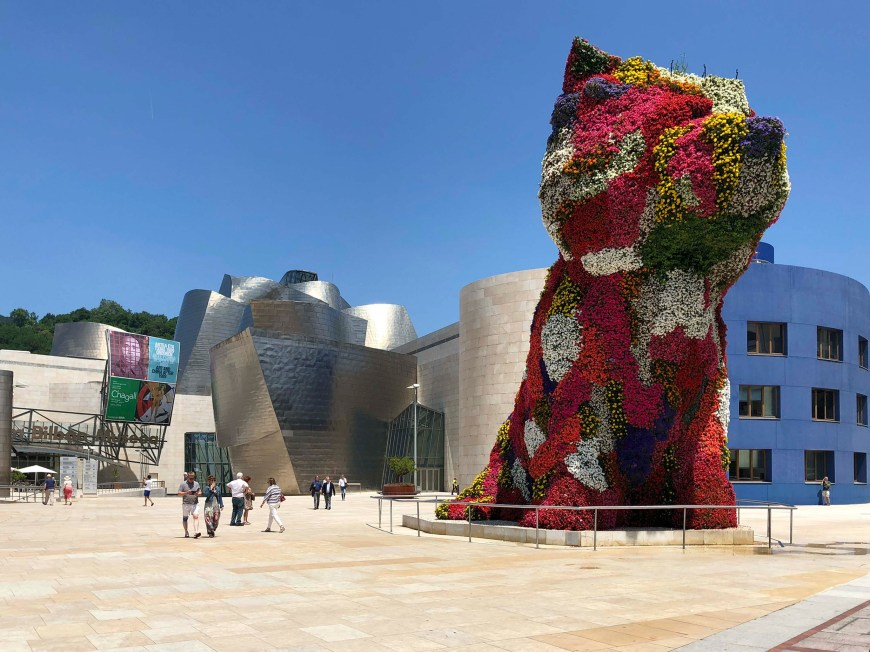
\includegraphics[width=\textwidth, height=6cm]{Figuras/Puppy.jpg}}
%En este caso, por propiedades de la imagen sleeccionada, esta es más alta y nuevamente ocupa el total de la minipágina.
\caption{Puppy - Guggenheim (Fuente: Google \cite{Puppy}).}
%Se incluye su subtítulo y su referencia.
\label{fig:Puppy}
%Se incluye su etiqueta.
\end{minipage}
%Se cierra el entorno de la minipágina.
\end{figure}
%Se cierra el entorno de la figura.

%Antes de acabar volvemos a la función "\vspace" que como se había visto anteriormente, se había saltado. Dicha función se utiliza para alinear verticalmente las dos imágenes. Como se puede observar, una es más alta que otra y esto implica que si no se utilizase "\vspace" (prueben a quitarlo), las fotos quedarían alineadas por el centro y no por su borde inferior. Así, se indica en la primera minipágina que esta comience 1.5 centímetros por debajo del entorno de la figura creada. Esto garantiza que las fotos se alineen por la parte inferior. Dicha medida de 1.5 centímetros variará en función de las dimensiones de las fotos y habrá que ajustarla manualmente para cada foto (al menos así lo he hecho yo, aunque seguramente haya otro método para hacerlo de forma automática, aunque yo personalmente lo desconozco).

%%%%%%%%%%%%%%%%%%%%%%%%%%%%%%%%%%%%%%%%%%%
%% FUNCIÓN PARA HACER LISTAS CON BULLETS %%
%%%%%%%%%%%%%%%%%%%%%%%%%%%%%%%%%%%%%%%%%%%

\begin{itemize}
%Esta función crea el entorno de enumeración. Al igual que antes se iniciaba el entorno figura, ahora es necesario iniciar el entorno para enumerar.

\renewcommand{\labelitemi}{$\bullet$}
%Esta función indica que se cambie el tipo marca para cada ítem del indicador por defecto al indicador con forma de bullet. Esto es por gusto personal y se pueden utilizar muchos otros indicadores (manos señalando, estrellas, cuadrados, bullets vaciados...). Para cambiar el indicador simplemente habrá de cambiar el parámetro "\bullet" por el correspondiente de los otros indicadores (su denominación se puede encontrar en los blogs referenciados al inicio de esta plantilla).

\setlength{\itemindent}{5mm}
%Esta función indica que cada ítem de la numeración se comience a escribir 5 milímetros más adentro respecto donde comienza a escribirse habitualmente el texto.

    \item Curabitur ullamcorper varius congue.
    %Función para crear cada uno de los ítem a enumerar.
    \item Vivamus eu quam sem. Aenean a ligula a est blandit dignissim vel non odio.
    \item Etiam sit amet velit quis enim porta semper sit amet vitae diam.

\end{itemize}
%Función para cerrar el entorno de enumeración

%%%%%%%%%%%%%%%%%%%%%%%%%%%%%%%%%&
%% INCLUIR UN PDF EN LA MEMORIA %%
%%%%%%%%%%%%%%%%%%%%%%%%%%%%%%%%%&

\includepdf[pages=2]{PDF/Prueba}
%Mediante esta función se puede incluir un PDF que se encuentre cargado en el menú del proyecto (izquierda). En el argumento obligatorio se incluirá la dirección en la que esté guardado el PDF y el nombre del mismo. En el argumento opcional se pueden incluir diferentes factores para personalizar la función. En este caso se ha incluido un parámetro que determina que únicamente se quiere incluir la página número 2 del documento.

%%%%%%%%%%%%%%%%%%%%%%%%%%%%%%%%%%%%%%%%%%%%%%%%%%%%%%%
%% FUNCIÓN PARA REFERENCIAR UN CAPÍTULO O UNA IMAGEN %%
%%%%%%%%%%%%%%%%%%%%%%%%%%%%%%%%%%%%%%%%%%%%%%%%%%%%%%%

\ref{fig:Gugg}
%La función como se puede observar es muy simple. Únicamente hay que incluir  en el parámetro obligatorio la etiqueta correspondiente a la imagen (o el capítulo) que se quiere referenciar. Así, en el texto aparecerá algo tal que asi: "Como se puede observar en la figura 1.2 ..." (Supuesto que 1.2 es el número asociado a la figura del Guggenheim).

%%%%%%%%%%%%%%%%%%%%%%%%%%%%%%%%%%%%%%%%%%%%%%%%%%%
%% FUNCIÓN PARA ESCRIBIR DE UN DETERMINADO COLOR %%
%%%%%%%%%%%%%%%%%%%%%%%%%%%%%%%%%%%%%%%%%%%%%%%%%%%

\textcolor{Rojo}{Como se puede observar en la imagen}
%Esta función simplemente permite escribir en un determinado color aquello que aparezca en el segundo argumento obligatorio. El primer argumento será el color en que se desea escribir y que ha de haber sido previamente definido.

%%%%%%%%%%%%%%%%%%%%%%%%%%%%%%%%%%%%%%
%% FUNCIÓN PARA ESCRIBIR EN NEGRITA %%
%%%%%%%%%%%%%%%%%%%%%%%%%%%%%%%%%%%%%%

\textbf{Descriptores}
%La función "\textbf" permite hace que el parámetro que se encuentra en su interior se escriba en negrita.

%%%%%%%%%%%%%%%%%%%%%%%%%%%%%%%%%%
%% FUNCIÓN PARA CREAR UNA TABLA %%
%%%%%%%%%%%%%%%%%%%%%%%%%%%%%%%%%%

%Quede por delante de esta función que en absoluto conozco la forma más óptima de realizar tablas. Únicamente incluí dos en mi memoria y la verdad que fue un proceso bastante costoso aún siendo estas considerablemente simples. Hay muchas información respecto a la creación de tablas en LATEX online y en caso de que se vayan a realizar tablas más complejas (de mayor tamaño, con combinación de celdas y demás) recomiendo encarecidamente profundizar más que lo que está presente en esta plantilla. De todos modos, ahí va todo lo que sé:

\renewcommand{\arraystretch}{1.6}
%Por cuestiones de gusto personal se ha restablecido el tamaño vertical de las celdas. Cambiado el valor se podrán hacer estas más grandes o más pequeñas.

\begin{table}[htbp]
%Con esta función se inicia el entorno tabla, que se puede posicionar con respecto al texto al igual que una imagen.

\begin{center}
%Se centra la tabla.

\begin{tabular}{|m{7cm}| m{7cm} |}
%Se inicia la creación de la tabla y se indica que se quiere que la distancia horizontal de cada celda sea de 7 centímetros. Además el parámetro "m" indica que se quiere el texto centrado en dichas celdas. Las barras "|" indica la separación entre una celda y otra. Es decir, estos símbolos son estrictamente las barras verticales que se deberían ver en la tabla.

\hline
%Mediante esta función se dibuja la línea horizontal que formará la primera linea de la tabla.

\rowcolor{Cyan}
%Mediante esta función se indica que el color de la primera fila será Cyan, evidentemente para que funcione habrá de estar previamente definido el color con sus dígitos RGB, como se ha explicado anteriormente.

\centering \textbf{Lorem ipsum} & \hspace{20pt}
%Estas funciones indican básicamente el texto a escribir en negrita y que de cara al siguiente texto se deja un espacio horizontal de 20 pt. El símbolo "&" indica el cambio a la celda contigua.

\textbf{dolor sit} \\\hline
%Nuevamente se introduce el texto de la segunda columna (todavía en primera fila) en negrita. Mediante las dos barras se indica que que se salta de fila y mediante "\hline" se indica que entre la fila 1 y la fila 2 haya una línea horizontal.

\textbf{consectetur adipiscing} & elit\\ \hline
\rowcolor{GrisTabla}
\textbf{consectetur adipiscing} & elit \\ \hline
\textbf{consectetur adipiscing} & Alta \\ \hline
\rowcolor{GrisTabla} 
\textbf{consectetur adipiscing} & elit \\ \hline
\textbf{consectetur adipiscing} & elit  \\ \hline
\rowcolor{GrisTabla} 
\textbf{consectetur adipiscing} & elit \\ \hline
\rowcolor{Naranja} 
\textbf{consectetur adipiscing} & \textbf{elit} \\ \hline
\end{tabular}
%Así, y del mismo modo, se van escribiendo todas las filas y columnas necesaria. Como se puede ver, se puede modificar a antojo el color de las filas o el texto de cada celda. 

\caption{Estudio resumen del impacto medioambiental (Fuente: Elaboración propia).}
%Función para incluir un subtítulo a la tabla.

\label{Medioambiente}
%Función para añadir una etiqueta a la tabla.

\end{center}
%Finalizar función de centrado de tabla.

\end{table}
%Función para salir del entorno tabla.


%%%%%%%%%%%%%%%%%%%%%%%%%%%%%%%%%%%%%%%%%%%%%%%%%%%%%%%%%
%% FUNCIÓN PARA CITAR UNA REFERENCIA DE LA BIBLIOGRAFÍA %%
%%%%%%%%%%%%%%%%%%%%%%%%%%%%%%%%%%%%%%%%%%%%%%%%%%%%%%%%%

\cite{Deusto}
%La función para citar esta también bastante simple. Simplemente se incluye en el argumento principal el nombre de la referencia a la que queramos llamar. Lógicamente para que esta referencia indique el número correspondiente debe existir un aparatado de bibliografía donde se ordenen y para elllo será también necesario contar con un archivos de referencias ".bib" cargado en el proyecto (menú izquierda).

%%%%%%%%%%%%%%%%%%%%%%%%%%%%%%%%%%%%%%%%%%%%%%%%%%%%%%%%%%%%%%%%%%
%% FUNCIÓN PARA GENERAR UNA BIBLIOGRAFÍA POR ORDEN DE APARICIÓN %%
%%%%%%%%%%%%%%%%%%%%%%%%%%%%%%%%%%%%%%%%%%%%%%%%%%%%%%%%%%%%%%%%%%

\bibliographystyle{unsrt}
%Lo primero de todo es definir el estilo de bibliografía que se va a utilizar. Concretamente este estilo "unsrt" ordena las referencias por el orden según se van enunciando a lo largo del texto. Se pueden utilizar muchos otros estilos para ordenar por ejemplo la bibliografía en orden alfabético, o para incluir el nombre del autor en minúscula y diversas otras propiedades. Es importante mirar cual es el formato que demandan las reglas de la memoria e intentar ajustarse con un estilo a este formato. Los distintos estilos se pueden encontrar a lo largo de los blogs comentados inicialmente. 

\bibliography{References.bib}
%Esta función es la que propiamente genera la bibliografía. Para crearla es importante llamar como argumento principal al archivo de referencias que se está utilizando. Dicho archivos será generalmente un archivo formato "bibtex", es decir ".bib". Para generar este tipo de archivos es altamente recomendable generarlos con un gestor de referencias y posteriormente exportarlos y subirlos al menú del proyecto. 

%A nivel personal recomiendo el gestor de referencias Mendeley, es gratis y funciona realmente bien tanto para libros como para referenciar páginas web. El gestor tiene un plug-in para Google Chrome para referenciar páginas web y además cuenta con aplicación de escritorio, lo que lo hace especialmente útil para trabajar. Hay otros gestores de referencias como RefWorks que para mi gusto personal no funcionan tan bien y fallan demasiado cuando son utilizados sobre páginas web, pero de todos modos si alguien ya está familiarizado con ellos los puede utilizar sin ningún problema pues también pueden generar los archivos .bib.

%Para acabar la lectura de esta plantilla, simplemente acuda al archivo "Refernces.bib". Queda muy poco.
